\documentclass[compress]{beamer}

\mode<presentation>
{
  \usetheme{Warsaw}
  % or ...
	\useoutertheme{infolines}
  \setbeamercovered{transparent}
  % or whatever (possibly just delete it)
}

\usepackage{verbatim}
\usepackage{listings}
\usepackage{tikz}
\usetikzlibrary{arrows}
\usetikzlibrary{shapes}
\tikzstyle{block}=[draw opacity=0.7,line width=1.4cm]

\lstloadlanguages{C++}
\lstnewenvironment{code}
	{%\lstset{	numbers=none, frame=lines, basicstyle=\small\ttfamily, }%
	 \csname lst@SetFirstLabel\endcsname}
	{\csname lst@SaveFirstLabel\endcsname}
\lstset{% general command to set parameter(s)
	language=C++, basicstyle=\footnotesize\sffamily, keywordstyle=\slshape,
	emph=[1]{tipo,usa}, emphstyle={[1]\sffamily\bfseries},
	basewidth={0.47em,0.40em},
	columns=fixed, fontadjust, resetmargins, xrightmargin=5pt, xleftmargin=15pt,
	flexiblecolumns=false, tabsize=2, breaklines,	breakatwhitespace=false, extendedchars=true,
	numbers=left, numberstyle=\tiny, stepnumber=1, numbersep=9pt,
	frame=l, framesep=3pt,
}

\usepackage[utf8]{inputenc}
\usepackage[T1]{fontenc}

% or whatever
\usepackage{fancyvrb}
\usepackage{times}
% Or whatever. Note that the encoding and the font should match. If T1
% does not look nice, try deleting the line with the fontenc.


\title[Búsqueda Binaria] % (optional, use only with long paper titles)
{Búsqueda Binaria}

\author[Quimey Vivas] % (optional, use only with lots of authors)
{Quimey Vivas \inst{1}\\ Leopoldo Taravilse \\ Facundo Gutierrez}
% - Give the names in the same order as the appear in the paper.
% - Use the \inst{?} command only if the authors have different
%   affiliation.
\institute[Avature] % (optional, but mostly needed)
{
  \inst{1}
  Avature Argentina
}
\date[TC 2018] % (optional, should be abbreviation of conference name)
{Training Camp 2018}

% Acá se puede insertar el logo de la UBA
% \pgfdeclareimage[height=0.5cm]{university-logo}{university-logo-filename}
% \logo{\pgfuseimage{university-logo}}



% Delete this, if you do not want the table of contents to pop up at
% the beginning of each subsection:
\AtBeginSubsection[]
{
  \begin{frame}<beamer>{Contenidos}
    \tableofcontents[currentsection,currentsubsection]
  \end{frame}
}


% If you wish to uncover everything in a step-wise fashion, uncomment
% the following command:

%\beamerdefaultoverlayspecification{<+->}
\fvset{fontsize=\scriptsize,numbersep=1mm,commandchars=\\\{\}}

\begin{document}
\pgfdeclarelayer{background}
\pgfsetlayers{background,main}
\begin{frame}
  \titlepage
\end{frame}

\begin{frame}{Contenidos}
  \tableofcontents
  % You might wish to add the option [pausesections]
\end{frame}

\section{Búsqueda Binaria discreta}

\subsection{Búsqueda binaria en un arreglo}

\begin{frame}{Buscando en listas ordenadas}
  \begin{itemize}
    \item Uno de los problemas más comunes que existen es el de querer buscar si un
          número aparece o no en una lista ordenada. \pause
    \invisible<1>{\item Es trivial ver que se puede resolver el problema en
          $O(n)$ donde $n$ es la cantidad de elementos de la lista, simplemente
          buscando uno por uno en orden.\pause
    }
    \invisible<1-2>{\item Hay una forma de aprovechar el hecho de que el arreglo
          está ordenado.
          Esta forma de buscar eficientemente se conoce como búsqueda binaria.
    }
  \end{itemize}
\end{frame}

\begin{frame}[fragile]{Ejemplo de Búsqueda Binaria}
  Supongamos que queremos buscar si el número 22 está en el siguiente arreglo:
  \begin{Verbatim}
  1 2 4 6 8 14 15 16 21 22 31 35 44 45 56 87 89 95 99 100 103 112 128
  \end{Verbatim}
  \pause
  \invisible<1>{
    Podemos preguntarnos
    ¿Es el primer elemento del arreglo el 22? No,
    ¿Es el segundo elemento del arreglo el 22?
    Tampoco... y así hasta que nos preguntamos
    ¿Es el décimo elemento del arreglo el 22? Sí!
  }
\end{frame}

\begin{frame}[fragile]{Ejemplo de Búsqueda Binaria}
  Con búsqueda binaria podemos buscar así
  \begin{Verbatim}
    \textbf{\textcolor{blue}{1}} 2 4 6 8 14 15 16 21 22 31 \textbf{\textcolor{red}{35}} 44 45 56 87 89 95 99 100 103 112 128 \textbf{\textcolor{blue}{.}}
  \end{Verbatim}
  \pause
  \begin{Verbatim}
    \textbf{\textcolor{blue}{1}} 2 4 6 8 \textbf{\textcolor{red}{14}} 15 16 21 22 31 \textbf{\textcolor{blue}{35}} 44 45 56 87 89 95 99 100 103 112 128
  \end{Verbatim}
  \pause
  \begin{Verbatim}
    1 2 4 6 8 \textbf{\textcolor{blue}{14}} 15 16 \textbf{\textcolor{red}{21}} 22 31 \textbf{\textcolor{blue}{35}} 44 45 56 87 89 95 99 100 103 112 128
  \end{Verbatim}
  \pause
  \begin{Verbatim}
    1 2 4 6 8 14 15 16 \textbf{\textcolor{blue}{21}} \textbf{\textcolor{red}{22}} 31 \textbf{\textcolor{blue}{35}} 44 45 56 87 89 95 99 100 103 112 128
  \end{Verbatim}
  \pause
  \invisible<1-4>{
    Notemos que en 4 pasos pudimos encontrar el 22 cuando
    antes nos llevaba 10 pasos.
  }
\end{frame}

\begin{frame}[fragile]{Código de la búsqueda binaria}
\begin{lstlisting}
# A es el arreglo ordenado, v es el valor a buscar
# Si v esta en A entonces esta en el intervalo [L, R) de A
def busqueda_binaria(A, v):
    L = 0
    R = len(A)
    while R - L > 1:
        M = (L + R) / 2
        if v < M:
            R = M
        else:
            L = M
    if A[L] == v:
        return L
    return None  # Not found
\end{lstlisting}
¿Funciona? ¿Encuentra la primera aparición de $v$? ¿La última? ¿Una cualquiera?


\end{frame}

\begin{frame}[fragile]{Ejemplo de Búsqueda Binaria}
Buscar un número que no está es mucho más costoso con búsqueda lineal,
sin embargo con búsqueda binaria es igual de rápido que buscar un número que
si está. Busquemos por ejemplo el 23.
\begin{Verbatim}
\textbf{\textcolor{blue}{1}} 2 4 6 8 14 15 16 21 22 31 \textbf{\textcolor{red}{35}} 44 45 56 87 89 95 99 100 103 112 128 \textbf{\textcolor{blue}{.}}
\end{Verbatim}
\pause
\begin{Verbatim}
\textbf{\textcolor{blue}{1}} 2 4 6 8 \textbf{\textcolor{red}{14}} 15 16 21 22 31 \textbf{\textcolor{blue}{35}} 44 45 56 87 89 95 99 100 103 112 128
\end{Verbatim}
\pause
\begin{Verbatim}
1 2 4 6 8 \textbf{\textcolor{blue}{14}} 15 16 \textbf{\textcolor{red}{21}} 22 31 \textbf{\textcolor{blue}{35}} 44 45 56 87 89 95 99 100 103 112 128
\end{Verbatim}
\pause
\begin{Verbatim}
1 2 4 6 8 14 15 16 \textbf{\textcolor{blue}{21}} \textbf{\textcolor{red}{22}} 31 \textbf{\textcolor{blue}{35}} 44 45 56 87 89 95 99 100 103 112 128
\end{Verbatim}
\pause
\begin{Verbatim}
1 2 4 6 8 14 15 16 21 \textbf{\textcolor{blue}{22}} \textbf{\textcolor{red}{31}} \textbf{\textcolor{blue}{35}} 44 45 56 87 89 95 99 100 103 112 128
\end{Verbatim}
\pause
\begin{Verbatim}
1 2 4 6 8 14 15 16 21 \textbf{\textcolor{blue}{22}} \textbf{\textcolor{blue}{31}} 35 44 45 56 87 89 95 99 100 103 112 128
\end{Verbatim}
\end{frame}

\begin{frame}{Complejidad de la búsqueda binaria}
La complejidad de la búsqueda binaria es $O(\log n)$ donde $n$ es el tamaño del
arreglo. Esto es fácil de probar ya que en cada paso se reduce el espacio de
búsqueda a la mitad.
\end{frame}

\subsection{Más allá de los arreglos}

\begin{frame}{Funciones monótonas}
Cuando tenemos una función $f$ que cumple
$$x > y \Rightarrow f(x) \geq f(y)$$
decimos que $f$ es monótona creciente. Si en cambio $f$ cumple
$$x > y \Rightarrow f(x) \leq f(y)$$
decimos que $f$ es monótona decreciente.
Si $f$ es monótona creciente o monótona decreciente decimos que $f$ es monótona.

Cuando una función es monótona creciente (decreciente) podemos aplicar
búsqueda binaria para buscar el menor valor de $x$ tal que
$f(x) \geq y$ ($f(x) \leq y$) para un $y$ dado.
\end{frame}

\begin{frame}{Ejemplo de búsqueda binaria con funciones monótonas}

Pedro estudia Ciencias de la Computación y le quedan por cursar $n$ materias.
Él sabe que si hace una sóla materia le va a costar 1 unidad de esfuerzo
aprobarla, pero si hace una segunda materia le cuesta 2 unidades de esfuerzo
para aprobar la segunda materia, y en general, si hace $i$ materias le cuesta
$i$ unidades de esfuerzo aprobar la $i$-ésima materia.

El sabe que hacer un esfuerzo de $t$ unidades o más lo va a estrezar y por lo
tanto va a dejar la carrera. Cuántos cuatrimestres necesita para recibirse?

\end{frame}

\begin{frame}{Ejemplo de búsqueda binaria con funciones monótonas}

\begin{itemize}
  \item Lo primero que tenemos que hacer es calcular cuántas materias puede
        hacer por cuatrimestre. Luego es una división.\pause
  \invisible<1>{\item Para calcular cuántas materias puede hacer por
    cuatrimestre, sabemos que ese número $x$ cumple con $\frac{x(x+1)}{2} < t$.
    Luego hacemos búsqueda binaria para encontrar ese máximo valor posible de
    $x$.
  }
\end{itemize}
\end{frame}
\section{Búsqueda binaria continua}

\subsection{Búsqueda binaria para el cálculo de funciones inversas}

\begin{frame}{Búsqueda binaria continua}
\begin{itemize}
  \item Así como usamos búsqueda binaria cuando tenemos un dominio discreto,
        también podemos usar búsqueda binaria cuando el dominio es continuo. \pause
  \invisible<1>{\item Por ejemplo, tenemos una función $f$ monótona creciente y
        continua y queremos hallar el mínimo $x$ tal que $f(x) \geq y$.
  }
  \pause
  \invisible<1-2>{\item Como $f$ es continua, si el mínimo $x_0$ existe tenemos
    qué $f(x_0) = y$, es decir $x_0 = f^{-1}(y)$.
  }
\end{itemize}
\end{frame}

\begin{frame}{Ejemplo de búsqueda binaria para encontrar el inverso de una función}
\begin{itemize}
  \item Dado un número $x$, calcular la raiz cuadrada de $x$ \pause
  \invisible<1>{
    \item ¿Cuál sería el criterio de terminación? ¿Cuántas iteraciones necesitamos?
  }\pause
  \invisible<1-2>{
    \item A diferencia del caso de la búsqueda binaria discreta, cuando el dominio
    de la búsqueda binaria es continuo tenemos que poner un punto de corte
    arbitrario para la búsqueda binaria.
  }
  \pause
  \invisible<1-3>{
    \item Podríamos cortar por ejemplo cuándo $R - L < 10^{-9}$ que nos da una
    precisión aceptable.
  }
  \pause
  \invisible<1-4>{
    \item Cuando el ciclo termina, tanto $L$ como $R$ contienen la respuesta con
    un error de a lo sumo $10^{-9}$.
  }
  \pause
  \invisible<1-5>{\item Método de Newton}
\end{itemize}
\end{frame}

\subsection{Búsqueda binaria con funciones de imagen booleana}

\begin{frame}{Búsqueda binaria con predicados booleanos}
\begin{itemize}
  \item Ya vimos como hace búsqueda binaria sobre funciones que tienen una
  imagen numérica y que son monotonas.
  \pause
  \invisible<1>{
    \item Cuando la imagen de la función es booleana, por ejemplo, dado un\
    predicado booleano $P$, encontrar el mínimo $x$ tal que $P(x)$ es verdadero,
    también podemos definir monotonía y aplicar búsqueda binaria.
  }
  \pause
  \invisible<1-2>{
    \item Cuando un predicado es falso para todos los $x < x_0$ y verdadero para
    los $x \geq x_0$ decimos que el predicado monótono.
    Esto equivale con asignarle $0$ a falso y $1$ a verdadero, en este caso el
    predicado es monótono creciente.
  }
\end{itemize}
\end{frame}
\section{Extras}
\subsection{Algunos comentarios}
\begin{frame}{}
  \begin{itemize}
    \item El caso no monónoto:
    \pause
    \invisible<1>{
    Si estamos tratando de encontrar $x$ tal que $f(x) = y$ y $f$ es continua
    podemos usar búsqueda binaria aunque $f$ no sea monónotona (por Bolzano).
    }
    \pause
    \invisible<1-2>{\item Sin cota superior:}
    \pause
    \invisible<1-3>{
      Si no tenemos una cota superior podemos usar búsqueda binaria para encontrarla.
    }
    \pause
    \invisible<1-4>{\item Búsqueda ternaria}
    \pause
    \invisible<1-5>{
      Si $f$ es \textit{unimodal} podemos usar búsqueda ternaria para encontrar el
      máximo (si $f$ no es unimodal encontramos un extremo local).
    }
    \pause
    \invisible<1-6>{\item Optimización $\Rightarrow$ Decisión}
  \end{itemize}
\end{frame}
\subsection{Ejemplos}
\begin{frame}{Ejemplo 1}
	\begin{block}{Máximo Cuadrado en un Tablero}
	Tenemos un tablero de $m \times n$ ($m$ filas y $n$ columnas).
  Algunas casillas del tablero están pintadas de blanco y otras de negro.
  Buscamos encontrar el tamaño del lado del subtablero cuadrado más grande de
  casillas negras.
	\end{block}
	\pause
	\invisible<1>{\begin{center}
		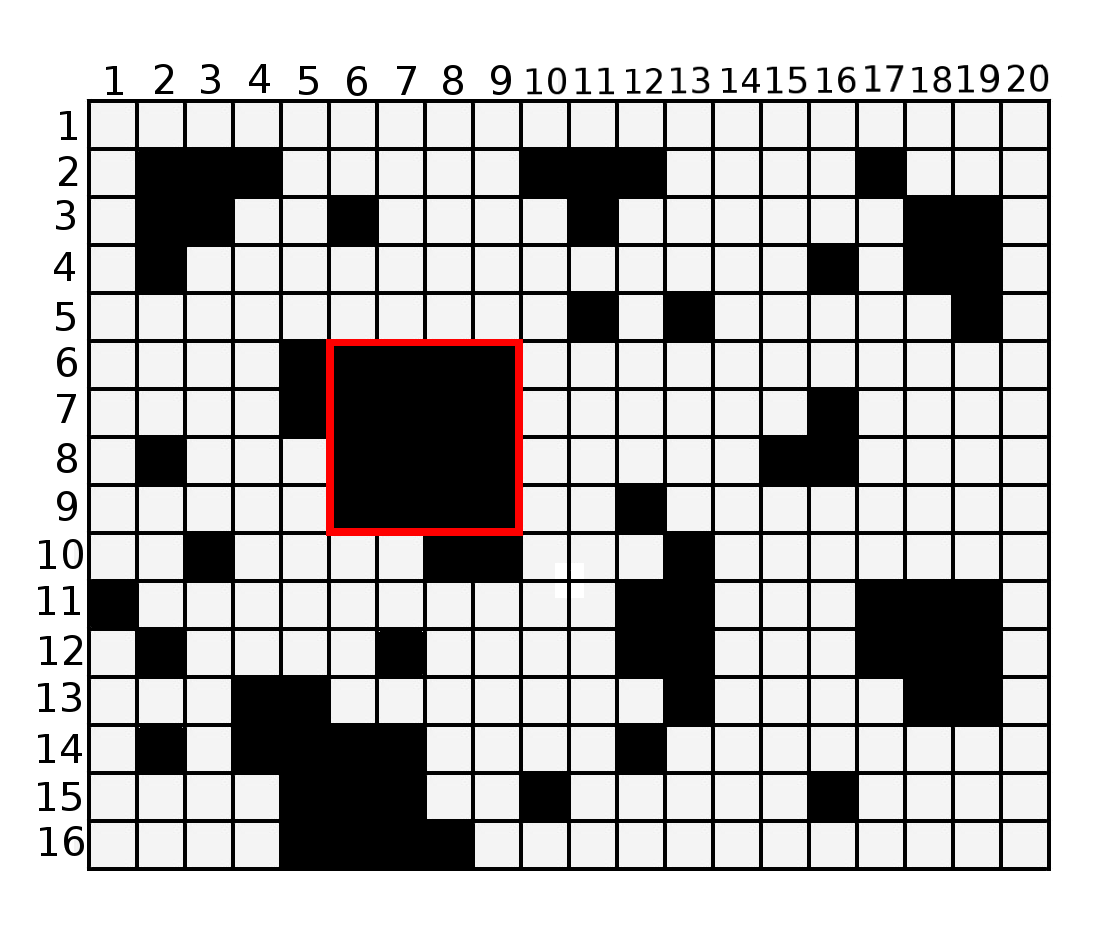
\includegraphics[scale=0.15]{tablero.png}
	\end{center}}
\end{frame}

\begin{frame}{Solución}
	\begin{block}{Cosas que vamos a usar}
		Supongamos que tenemos una función booleana $f(k,i,j)$ que
    \textbf{nos dice si hay un cuadrado de casillas negras de lado $k$}
    en el tablero cuya casilla superior izquierda está situada en la fila $i$
    y la columna $j$.
    Por ejemplo, en la imagen anterior, $f(2,2,2)$ es \texttt{true} y
    $f(3,2,2)$ es \texttt{false}.
	\end{block}
	\pause
  {\fontsize{9.5pt}{11.4pt}
	\begin{enumerate}
		\invisible<1>{\item Solución:
    Podemos \textbf{recorrer todas las casillas}, y en cada una preguntarle a
    la función $f$ si existe un tablero de tamaño $0,1,2,\dots, \text{min}(n,m)$
    inclusive. El valor más grande que devolvió \texttt{true} será el lado del
    cuadrado más grande que tiene la esquina superior izquierda en la casilla
    que estamos analizando. Tomando el máximo de este número para todas las
    casillas resolvemos el problema.}
		\pause
		\invisible<1-2>{¿Cuántas veces estamos llamando a la función $f$?}
		\pause
		\invisible<1-3>{
      \underline{Respuesta} : $\boxed{n\cdot m \cdot \text{min}(n,m) \sim n^3}$
    }
	\end{enumerate}
  }
\end{frame}

\begin{frame}{Solución}
	¿Cómo podemos \textbf{acelerar la solución}? (hacer menos llamados a la $f$)
	\pause

	\invisible<1>{\textbf{Búsqueda binaria}}
	\pause
  \invisible<1-2>{Ok... ¿Pero en qué?}
	\pause
	\begin{enumerate}
		\setcounter{enumi}{1}
		\invisible<1-3>{
      \item En la solución anterior, cuando estamos parados en una casilla,
      podemos hacer búsqueda binaria en \textbf{el lado del cuadrado que buscamos}.
    }
	\end{enumerate}
	\pause
	\invisible<1-4>{¿Cuántas veces estamos llamando a la función $f$?}
	\pause

	\invisible<1-5>{
    \underline{Respuesta} :
    $\boxed{n\cdot m \cdot \lg \left (\text{min}(n,m)\right ) \sim n^2 \cdot \lg(n)}$
  }
\end{frame}
\begin{frame}{Ejemplo 2}
\begin{block}{Problema}
Fito tiene que cruzar un cuarto lleno de dinosaurios desde la esquina superior
izquierda hasta la esquina inferior derecha. Son dadas las posiciones de los
dinosaurios y las dimensiones del cuarto.
Se sabe que si pasa a distancia menor a $T$ de un dinosaurio, este lo ve y se
lo come. Cuál es el mínimo $T$ tal que Fito puede lograr su objetivo?
\end{block}
\end{frame}
\section{Ventanas Deslizantes}
\subsection{Ejemplos}
\begin{frame}
	\begin{block}{Problema:}
	Dado un arreglo de $n$ números \textbf{positivos}, y un número $x$, nos
  interesa saber si existe un subarreglo cuya suma sea $x$.
	\end{block}
	\pause
	\begin{block}{Ejemplos:}
   		\begin{itemize}

			\item $A = [2, 3, 2, 5, 1, 5, 2, 3]$. Buscamos sumar $ x = 8$

			La respuesta es : \pause "El subarreglo $[2..4]$ suma $8$"
			\pause
			\item $A = [2, 3, 2, 5, 1, 5, 2, 3]$. Buscamos sumar $ x = 4$

			La respuesta es : \pause "No hay subarreglo de $A$ que sume $4$"
		\end{itemize}
	\end{block}
\end{frame}
\begin{frame}{Solución}
	\begin{enumerate}
		\item \textbf{Probar todos los subarreglos posibles}.
    Es decir, todos los subarreglos $[i..j]$ con $0 \leq j < n$ e $ 0 \leq i \leq j$.
    Para cada uno de ellos calcular \texttt{suma}(i,j),
    la suma de los números en el subarreglo especificado y ver si es exactamente $x$.

		Complejidad :
    \pause
    \invisible<1> {
      $\mathcal{O}(n^3)$ u $\mathcal{O}(n^2)$ dependiendo de la implementación de la función \texttt{suma}.
    }
		\pause
		\invisible<1-2>{
      \item Utilizar una \textbf{ventana deslizante} para resolver el problema.
      La idea es mantener \textbf{dos índices} que son los extremos de nuestra
      ventana deslizante, al extremo izquierdo lo llamaremos "$i$" y al derecho
      lo llamaremos "$j$".
		  Ambos extremos comienzan en el principio del arreglo, y en todo momento
      vamos a \textbf{mantener} cuánto vale
      \textbf{la suma de los números dentro de la ventana [i..j)}
      (notar que no incluimos el extremo derecho).
    }
	\end{enumerate}
\end{frame}
\begin{frame}{Análisis}
	\begin{itemize}
		\item ¿Cuántos pasos hace el algoritmo?
    \underline{Respuesta} : \pause
		\invisible<1>{
       En cada paso, o bien \textbf{aumenta i} o \textbf{aumenta j}.
       Cada uno de ellos puede ser aumentado a lo sumo $n$ veces.
       Por lo tanto al cabo de \textbf{$2n$ pasos} en el peor caso,
       finaliza nuestro algoritmo.
     }
		\pause
    \invisible<1-2>{
		  \item ¿Por qué es importante que los números sean \textbf{positivos}?
      \underline{Respuesta} :
    }
		\pause
    \invisible<1-3>{
      Porque nos permite saber que si en algún momento $\texttt{suma} > x$,
      entonces todas las ventanas que tienen el mismo valor de $i$ y un $j$
      mayor tendrán una suma mayor y podemos no mirarlas
      (de alguna forma, podemos afirmar que \textbf{"ya nos pasamos"}).
    }
	\end{itemize}
\end{frame}
\begin{frame}{2SUM}
	\begin{block}{Problema:}
	Dado un arreglo de $n$ números, y un número $x$. Queremos encontrar dos números del arreglo que sumen $x$, o reportar que no existe tal par.
	\end{block}
	\pause
	\begin{block}{Ejemplos:}
   		\begin{itemize}
			\item $A = [7,10,4,1,9,5,9,6]$. Buscamos sumar $ x = 12$
			La respuesta es : \pause "Sumando $A[0]$ y $A[5]$ obtenemos $12$"
			\pause
			\item $A = [7,10,4,1,9,5,9,6]$. Buscamos sumar $ x = 4$
			La respuesta es : \pause "No hay dos elementos de $A$ que sumen $4$"
		\end{itemize}
	\end{block}
\end{frame}

\begin{frame}{Solución}
	\begin{block}{Observación clave}
		Es importante notar que el orden de los números en el arreglo A no juega ningún rol. Entonces podemos asumir que tienen el orden que nos convenga. En particular, podemos asumir que el arreglo está \textbf{ordenado en forma creciente} (u ordenarlo en $\mathcal{O}(n \lg(n))$ )
	\end{block}
	\pause
	\begin{enumerate}
		\invisible<1>{
      \item Probar todos los pares de índices, y ver si esos dos números suman
      o no $x$. De existir un par que sí, reportarlo.
      Complejidad $\mathcal{O}(n^2)$
    }
		\pause
		\invisible<1-2>{
      \item Utilizar una variante de la técnica que vimos recién para resolver
      el problema. En lugar de tener dos índices que siempre aumentan, ahora
      tendremos dos índices.
      \textbf{Uno siempre aumenta, el otro siempre disminuye}.
      Por lo tanto también haremos \textbf{a lo sumo 2n pasos}.
      Complejidad $\mathcal{O}(n)$.
    }
    \pause
    \invisible<1-3>{
      \item Búsqueda binaria, hashmap, \dots
    }
	\end{enumerate}
\end{frame}
\begin{frame}{K-ésima distancia entre puntos de la recta}
	\begin{block}{Problema:}
		Dados n puntos en la recta numérica ($x_1, x_2, \dots, x_n$), y un número $k$. Si listamos todas las distancias entre pares de puntos ($x_i,x_j$) con $i < j$ y ordenamos estas distancias (puede haber repetidas). Queremos saber qué distancia queda en el k-ésimo lugar.
	\end{block}
	\begin{center}
		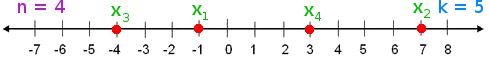
\includegraphics[scale=0.5]{recta.png}
	\end{center}
	\pause
  \vspace{-25pt}
	\begin{columns}[t]
        \begin{column}{.3\textwidth}
			{\footnotesize
			\begin{enumerate}
				\item	$\text{dist}(x_1,x_2) = 8$
				\item	$\text{dist}(x_1,x_3) = 3$
				\item	$\text{dist}(x_1,x_4) = 4$
				\item	$\text{dist}(x_2,x_3) = 11$
				\item	$\text{dist}(x_2,x_4) = 4$
				\item	$\text{dist}(x_3,x_4) = 7$
			\end{enumerate}
			}
        \end{column}
        \pause
        \begin{column}{.7\textwidth}
        {\Huge
            $$ D = [3,4,4,7,8,11] $$
        }
        \end{column}
    \end{columns}
\end{frame}

\begin{frame}{Solución}
	\begin{enumerate}
		\item Calcular todas las distancias, ordenarlas, y ver qué elemento está en
    el $k$-ésimo lugar. Complejidad : $\mathcal{O}(n^2 + n^2 \lg(n^2))$
		\pause
    \invisible<1> {
		\item Usar \textbf{Binary Search} y una \textbf{Ventana deslizante}.
    }
		\pause
    \invisible<1-2>{
      Haremos búsqueda binaria en la distancia. Formalmente, la propiedad será:

		  {\small $P(d) : \text{La cantidad de distancias menores que \textbf{d} es menor que k}$}
    }
		\pause
    \invisible<1-3>{
		  Ordenados los puntos, para una \textbf{distancia $d$ fija},
      podemos ir moviendo una ventana deslizante que
      \textbf{
        para cada extremo izquierdo nos diga cuántos puntos están a distancia menor que $d$
      }.
    }
		\pause
    \invisible<1-4> {
		  Complejidad :
        $\mathcal{O} (\underbrace{n \lg(n)}_{\text{Ordenar}} + \underbrace{\lg(n)}_{\text{BB}} \cdot \underbrace{n}_{\text{VD}}) = \mathcal{O} (n \lg(n))$
    }
	\end{enumerate}
\end{frame}
\begin{frame}{Tarea}
  \begin{itemize}
    \item \url{http://codeforces.com/problemset/problem/760/B}
    \item \url{https://icpcarchive.ecs.baylor.edu/external/44/4478.pdf}
    \item \url{https://www.spoj.com/problems/TAP2015B/}
    \item \url{http://www.spoj.com/problems/DINOSM/}
  \end{itemize}
\end{frame}
\end{document}
